\documentclass[letterpaper,12pt,notitlepage]{article}

%\usepackage{syntonly}
%\syntaxonly

%\usepackage[UTF8]{ctex}

%\usepackage{ctex}
\usepackage[english]{babel}
\usepackage{graphicx}
\usepackage{fancyhdr}
\usepackage{lipsum}
\usepackage{geometry}
\usepackage{amsmath}
\usepackage{subcaption}
\usepackage{comment}
\usepackage{pdfpages}

\renewcommand{\familydefault}{\sfdefault}
%\usepackage{fontspec}
%\setmainfont{Times New Roman}

\geometry{margin=1in}

\pagestyle{fancy}

\fancyhf{}

\renewcommand{\headrulewidth}{0.5pt}
\renewcommand{\footrulewidth}{0.2pt}

\fancyhead[c]{ELEX-4560-0 - Telecom \& Networks Project}
\fancyfoot[r]{\thepage}
\fancyfoot[L]{\jobname}
%E: Even page O: Odd page L left C center R right H header F footer

\setlength{\headheight}{15pt} 





\begin{document}
\begin{titlepage}
	\vspace{5cm}
	\begin{center}
		
\includegraphics[scale=0.4]{bcit.png}\\

		\huge{ELEX-4560-0 - Telecom \& Networks Project}\\
		\vspace{10mm}
		\large{\textbf{Preliminary Design}}\\
		\vspace{10mm}
		\large{Tianze Wu}\\
		\vspace{5mm}
		Inhee Hwang\\
		\vspace{5mm}
		\today

	\end{center}
\end{titlepage}

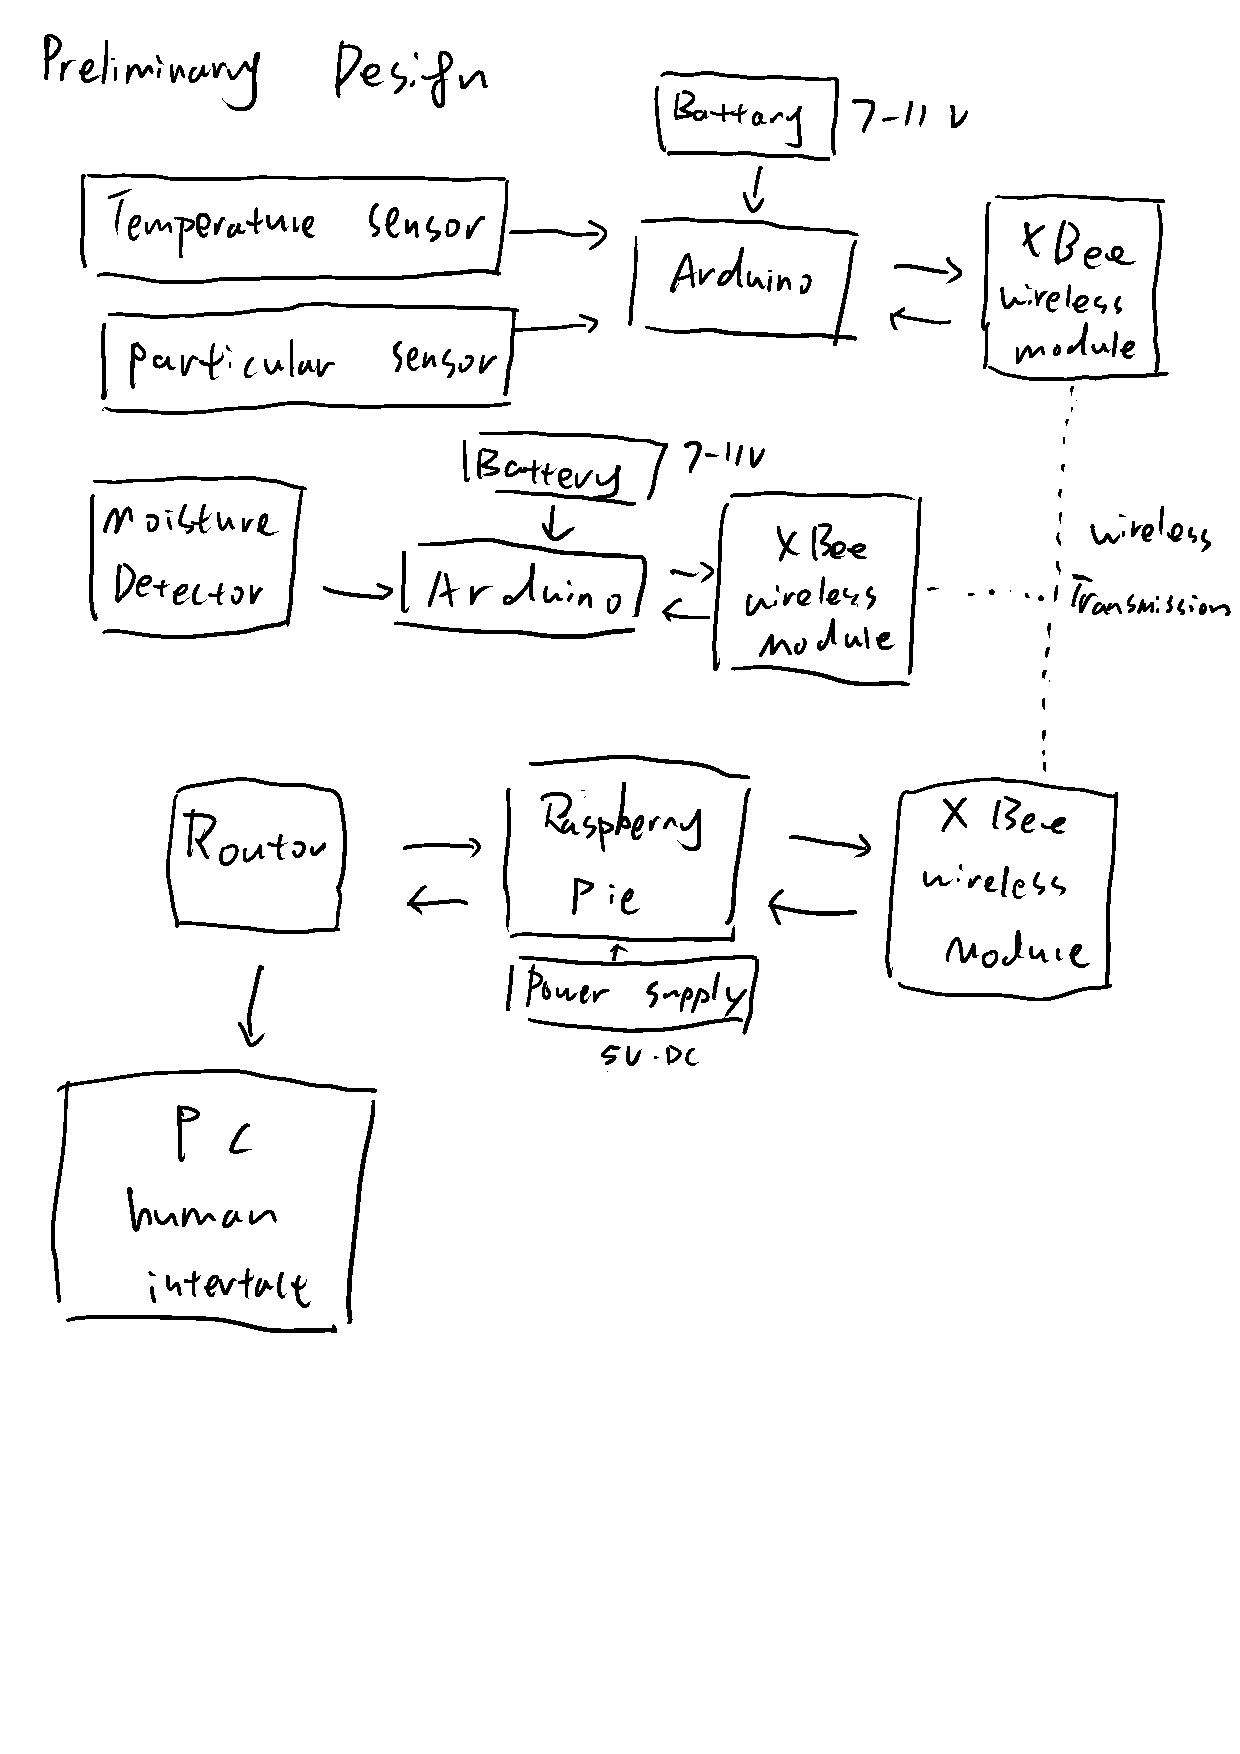
\includepdf[pages=1]{Preliminary_Design_Draft.pdf}
\clearpage 
\section*{Descreption}
\par There are 13 blocks including 3 power supplies, 3 sensors, 3 wireless modules, 
two arduinos, one Raspberry Pie and human interfaces. For the connection between Raspberry Pie 
and PC, we can use a USB wire or wifi(by router). Two power supplies(battery) use the 
voltage between 7V to 11V(required by Arduino) and one 5V(required by Raspberry Pie). 
The transimssion meida between XBee is air and the range of operation is lees than 100ft. 



\end{document}



\begin{comment}

	\begin{figure}[ht!]
		\centering
		\begin{subfigure}[b]{0.45\textwidth}
			\includegraphics[width = \textwidth]{pic.jpg}
			\caption{Differentiate Sine Wave}
		\end{subfigure}
		\begin{subfigure}[b]{0.45\textwidth}
			\includegraphics[width = \textwidth]{pic.jpg}
			\caption{Differentiate Triangle Wave}
		\end{subfigure}
	\end{figure}
	
	\includegraphics[width = \textwidth]{pic.jpg}
	
	example of picture 
	
	\begin{table}[ht!]
		\centering
		\begin{tabular}{ |c |c |}
			\hline
			Parameter & Measured with RCL Meter \\
			\hline
			Capacitance [µF] & 25.78 \\
			\hline
			Inductance [µH] &  60.58\\
			\hline
		\end{tabular}
		\caption{Cable Capacitance and Inductance Measurements (RCL Meter)}
	\end{table}
	Example of table
	\end{comment}
